\documentclass[12pt]{article}
\usepackage{amsmath}
\usepackage{graphicx}
\usepackage{pdfpages}

\title{Exercise Set 1}
\author{Ryan C. Bleile}

\begin{document}
\maketitle

\section{}
Our operator T() and function domain f is:
$$ T(f) = 2f + \frac{df}{dt} + 2\frac{d^{2}f}{dt^{2}} $$
$$ f = a\ cos(wt) + b\ sin(wt) \equiv (a,b)$$

In order to find a solution to the operator T(), for T(a,b), we must perform the operation once with calculus to get a solution in the (a,b) form. So solving for T(f) gives:

\begin{eqnarray*}
T(f) 	&=&	2a\ cos(wt) + 2b\ sin(wt) - aw\ sin(wt) + bw\ cos(wt) - 2aw^{2}\ cos(wt) - 2bw^{2}\ sin(wt)\\
		&=&	(2a + bw - 2aw^{2})\ cos(wt) + (2b - aw - 2bw^{2})\ sin(wt)\\
		&=& (a(2-2w^{2}) + b(w)\ cos(wt) + (a(-w) + b(2-2bw^{2}))\ sin(wt)\\
\end{eqnarray*}
This yields the result that in terms of the input point (a,b): 
\begin{eqnarray*}
T(a,b)	&=& ( a(2-2w^{2}) + b(w) , a(-w) + b(2-2w^{2}) ) 
\end{eqnarray*}

With this equation for the solution to the operator T in this domain we are able to solve any number of sets of T operators for any inputs a and b. To solve for $T^{2}(a,b)$ we will use the solution we obtained for T(a,b) and plug it back into itself. Consider T(a,b) = (A,B) and now we will find T(A,B) from our equation derived above.

\begin{eqnarray*}
T^{2}(a,b) 	&=& T(A,B)\\
T(A,B) 		&=& ( A(2-2w^{2}) + B(w)) , A(-w) + B(2-2w^{2}) )\\
			&=& ( (a(2-2w^{2}) + b(w))(2-2w^{2}) + (a(-w) + b(2-2w^{2}))(w)) , (a(2-2w^{2}) + b(w))(-w) + (a(-w) + b(2-2w^{2}))(2-2w^{2}) )\\
			&=&	( a(4 - 7w^{2} + 4w^{4})) + b(4w - 4w^{2}) , a(4w - 4w^{2}) + b(4 - 7w^{2} + 4w^{4}) ) 
\end{eqnarray*}

\section{}

Beginning with a new operator S() defined such that:
$$ S(f) = 2f + \frac{df}{dt} + \frac{d^{2}f}{dt^{2}} $$
where f is defined as in the previous problem to be:
$$ f = a\ cos(wt) + b\ sin(wt) \equiv (a,b)  $$
In order to find a solution to the operation in terms of the inputs (a,b) we will need to solve it one time in terms of the calculus solution. Doing so yields:

\begin{eqnarray*}
S(f) 	&=&	2a\ cos(wt) + 2b\ sin(wt) - aw\ sin(wt) + bw\ cos(wt) - aw^{2}\ cos(wt) - bw^{2}\ sin(wt)\\
		&=&	(2a + bw - aw^{2})\ cos(wt) + (2b - aw - bw^{2})\ sin(wt)\\
		&=& (a(2-w^{2}) + b(w)\ cos(wt) + (a(-w) + b(2-bw^{2}))\ sin(wt)
\end{eqnarray*}
This yields the result in terms of (a,b) as:

$$ S(a,b) = ( a(2-w^{2}) + b(w) , a(-w) + b(2-w^{2}) )  $$

Now we can use S(a,b) to solve for a combination of circuits, T(S(a,b)) and S(T(a,b)). If we write T(a,b) = (A,B) and S(a,b) = (C,D) than we are able to rewrite the equations for T(S(a,b)) as T(C,D) and S(T(a,b)) as S(A,B). So solving first for T(C,D) we find that:

\begin{eqnarray*}
T(C,D)	&=&	( C(2-2w^{2}) + D(w) , C(-w) + D(2-2w^{2}) )\\
		&=& ( (a(2-w^{2}) + b(w))(2-2w^{2}) + (a(-w) + b(2-w^{2}))(w) , (a(2-w^{2}) + b(w))(-w) + (a(-w) + b(2-w^{2}))(2-2w^{2}) )\\
		&=& ( a(4 - 7w^{2} + 2w^{4}) + b(4w - 3w^{3}) , a(-4w+3w^{3}) + b(4-7w^{2}+2w^{4}) )
\end{eqnarray*}

This results in the equation for the Solution of T(S(a,b)) in terms of the two inputs (a,b) is then:

$$ T(S(a,b)) = ( a(4 - 7w^{2} + 2w^{4}) + b(4w - 3w^{3}) , a(-4w+3w^{3}) + b(4-7w^{2}+2w^{4}) ) $$

Now we will solve the S(T(a,b)) using S(A,B):

\begin{eqnarray*}
S(A,B)	&=&	( A(2-w^{2}) + B(w) , A(-w) + B(2-w^{2}) )\\
		&=&	( (a(2-2w^{2}) + b(w))(2-w^{2}) + (a(-w) + b(2-2w^{2}))(w) , (a(2-2w^{2}) + b(w))(-w) + (a(-w) + b(2-2w^{2}))(2-w^{2}) )\\
		&=&	( a(4 - 7w^{2} + 2w^{4}) + b(4w-3w^{3}) , a(-4w+3w^{3}) + b(4-7w^{2}+2w^{4}) )
\end{eqnarray*}

Giving us a result for S(T(a,b)) to be:

$$ S(T(a,b)) =  a(4 - 7w^{2} + 2w^{4}) + b(4w-3w^{3}) , a(-4w+3w^{3}) + b(4-7w^{2}+2w^{4}) $$

From this we see that both S(T(a,b)) and T(S(a,b)) yield the same result meaning that we can apply the transformation in any order to get the same result, just like any linear operation.

\section{}

Using a Perl script to preform the operations for S as defined above for $S^{n}(1,1)$ from n = 1 to 10 we see that it performs a spiral operation on the points in the plane; as shown bellow. This operation is both a rotation and an expansion of the points of the plane. Also shown below is the plots of (1,2), (2,1), and (2,2) to show the effect. with w values of 1, 2 and 3.  

\begin{figure}[h!]
  \caption{a = 1, b = 1, w = 1}
  \centering
    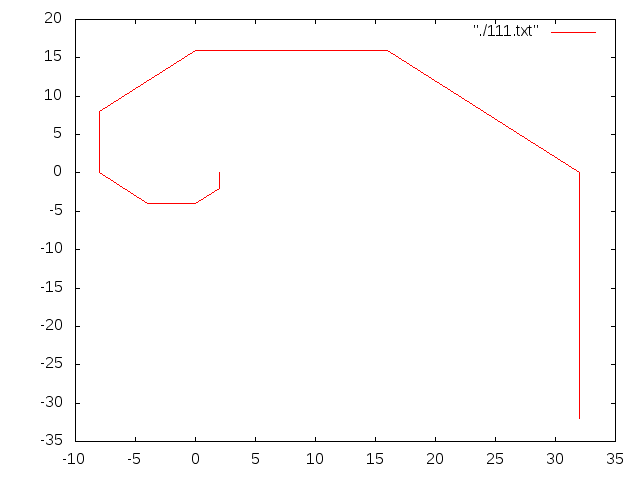
\includegraphics[scale=0.3]{111.png}
\end{figure}
\begin{figure}[h!]
  \caption{a = 1, b = 1, w = 2}
  \centering
    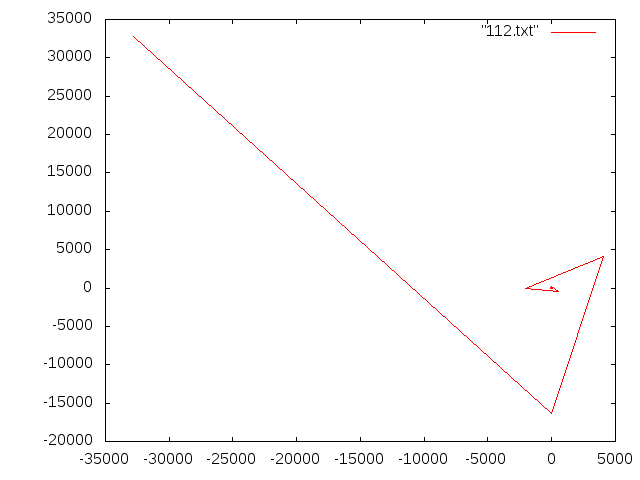
\includegraphics[scale=0.3]{112.png}
\end{figure}
\begin{figure}[h!]
  \caption{a = 1, b = 1, w = 3}
  \centering
    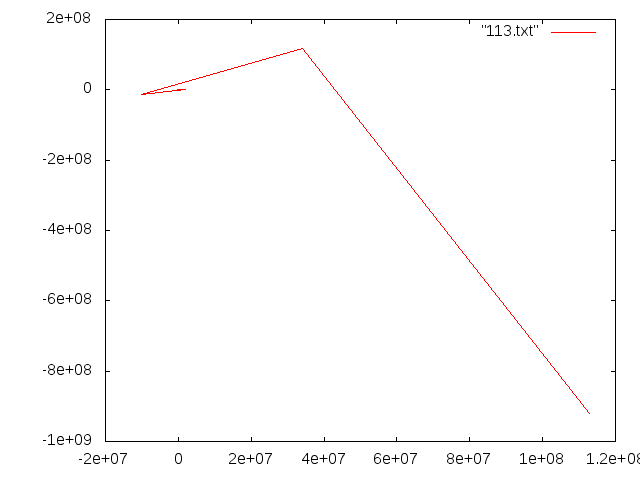
\includegraphics[scale=0.3]{113.png}
\end{figure}
\begin{figure}[h!]
  \caption{a = 1, b = 2, w = 1}
  \centering
    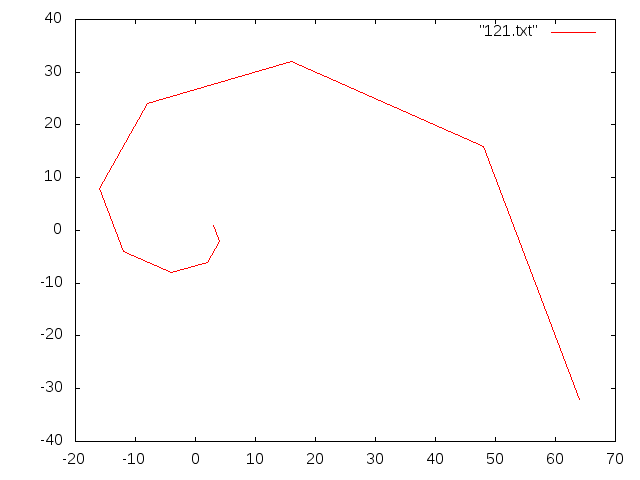
\includegraphics[scale=0.3]{121.png}
\end{figure}
\begin{figure}[h!]
  \caption{a = 1, b = 2, w = 2}
  \centering
    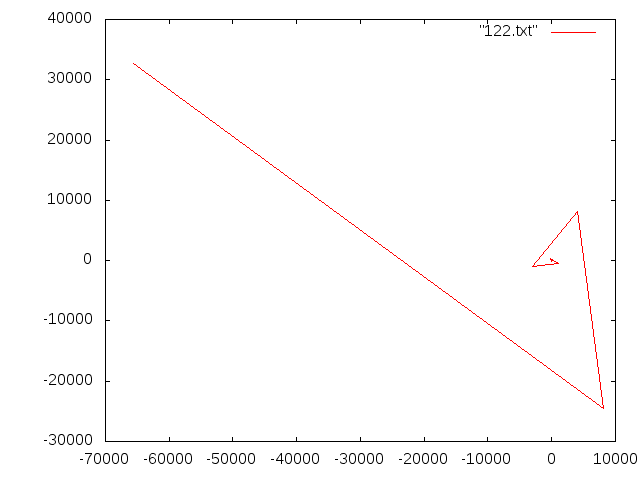
\includegraphics[scale=0.3]{122.png}
\end{figure}
\begin{figure}[h!]
  \caption{a = 1, b = 2, w = 3}
  \centering
    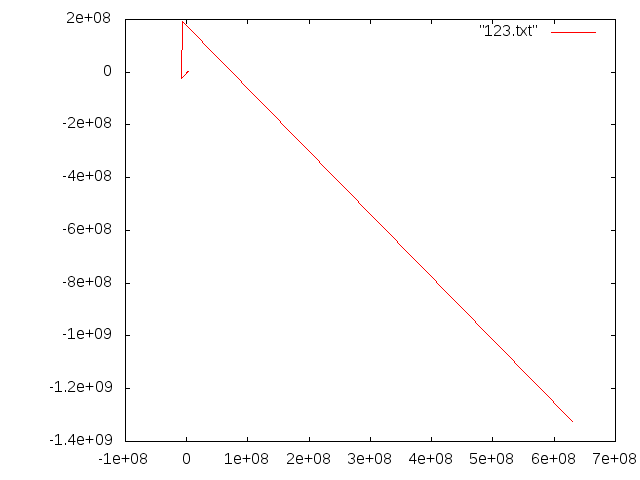
\includegraphics[scale=0.3]{123.png}
\end{figure}
\begin{figure}[h!]
  \caption{a = 2, b = 1, w = 1}
  \centering
    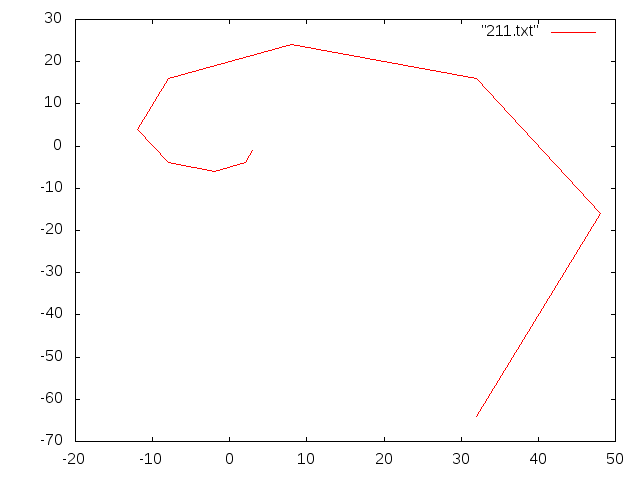
\includegraphics[scale=0.3]{211.png}
\end{figure}
\begin{figure}[h!]
  \caption{a = 2, b = 1, w = 2}
  \centering
    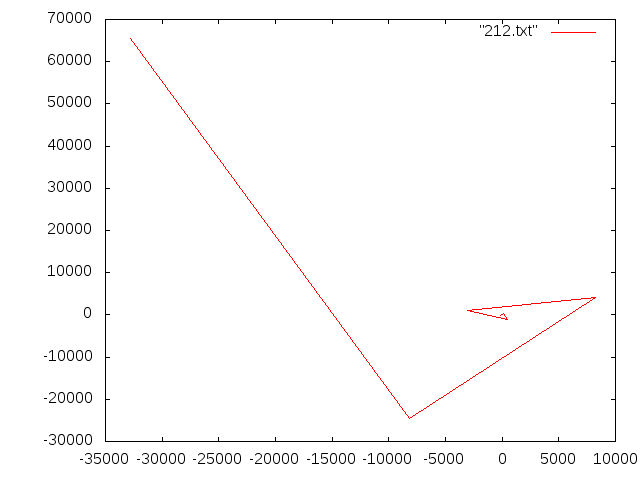
\includegraphics[scale=0.3]{212.png}
\end{figure}
\begin{figure}[h!]
  \caption{a = 2, b = 1, w = 3}
  \centering
    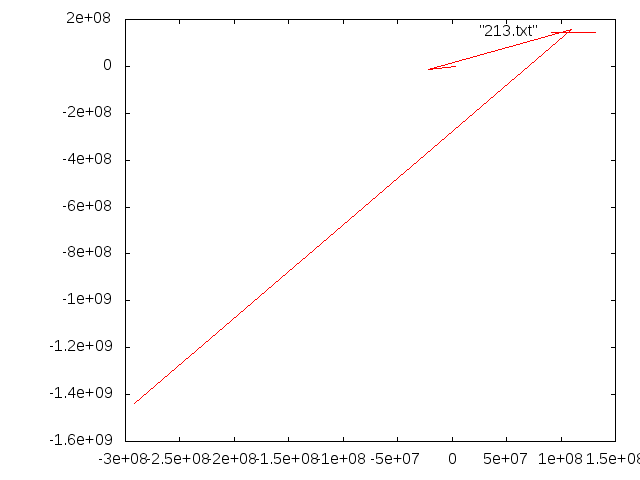
\includegraphics[scale=0.3]{213.png}
\end{figure}
\begin{figure}[h!]
  \caption{a = 2, b = 2, w = 1}
  \centering
    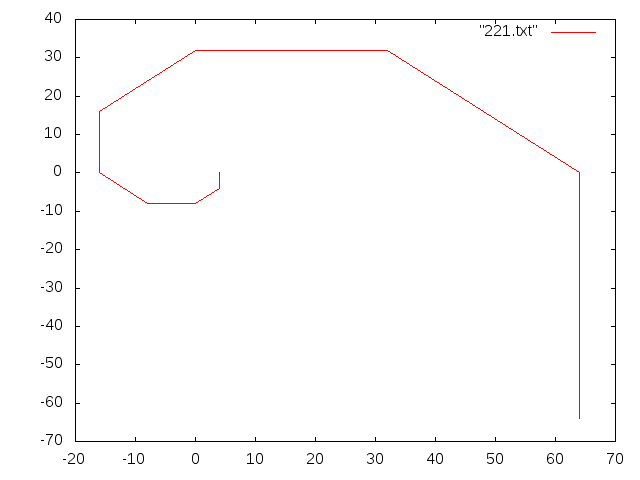
\includegraphics[scale=0.3]{221.png}
\end{figure}
\begin{figure}[h!]
  \caption{a = 2, b = 2, w = 2}
  \centering
    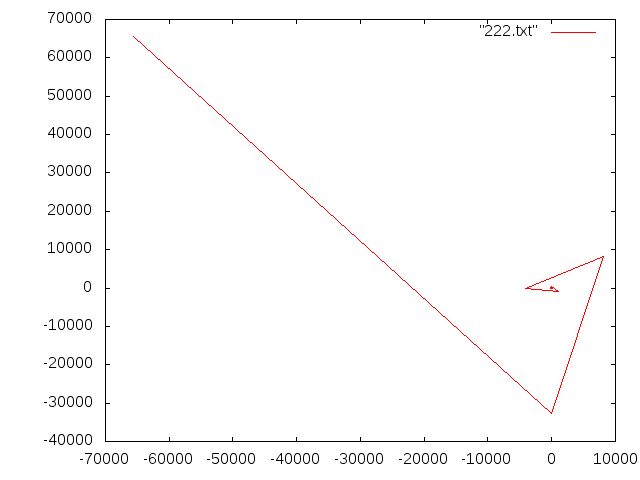
\includegraphics[scale=0.3]{222.png}
\end{figure}
\begin{figure}[h!]
  \caption{a = 2, b = 2, w = 3}
  \centering
    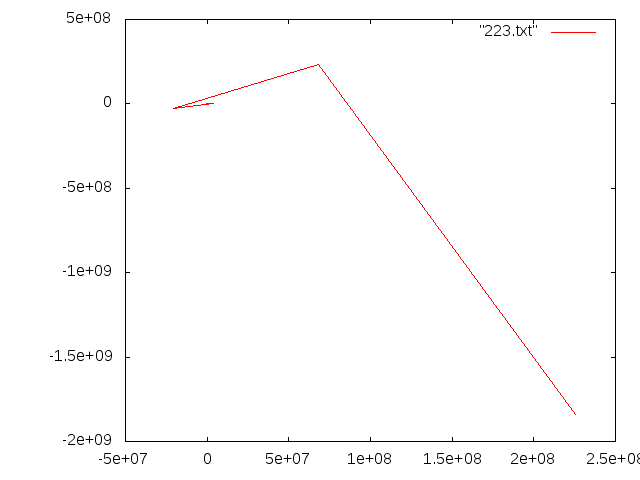
\includegraphics[scale=0.3]{223.png}
\end{figure}
\newpage
$S^{-1}(a,b)$ is the inverse operation to that of S(a,b). To perform the inverse operation instead of multiplying the a and b terms one would have to divide them. This would produce an undefined divide by zero, or the b term would go to infinity; for any case in which one of the S(a,b) terms would have normally gone to 0 the inverse operation is going to be undefined.  
$$ S^{-1}(a,b) = ( \frac{a}{ a(2-w^{2}) + b(w)} , \frac{b}{a(-w) + b(2-w^{2})} ) $$

so $S^{-1}(1,1)$ equals ($\frac{1}{2}$, $\frac{1}{0}$)

\end{document}